% !TEX TS-program = pdflatex
% !TEX encoding = UTF-8 Unicode

% This is a simple template for a LaTeX document using the "article" class.
% See "book", "report", "letter" for other types of document.

\documentclass[11pt]{article} % use larger type; default would be 10pt

\usepackage[utf8]{inputenc} % set input encoding (not needed with XeLaTeX)

%%% Examples of Article customizations
% These packages are optional, depending whether you want the features they provide.
% See the LaTeX Companion or other references for full information.

%%% PAGE DIMENSIONS
\usepackage{geometry} % to change the page dimensions
\geometry{top=2cm,bottom=2cm,left=2cm,right=2cm,letterpaper} % or letterpaper (US) or a5paper or....

\usepackage{graphicx} % support the \includegraphics command and options

% \usepackage[parfill]{parskip} % Activate to begin paragraphs with an empty line rather than an indent

%%% PACKAGES
\usepackage{booktabs} % for much better looking tables
\usepackage{array} % for better arrays (eg matrices) in maths
\usepackage{paralist} % very flexible & customisable lists (eg. enumerate/itemize, etc.)
\usepackage{epsfig}
\usepackage{verbatim} % adds environment for commenting out blocks of text & for better verbatim
\usepackage{subfig} % make it possible to include more than one captioned figure/table in a single float
\usepackage{amstext}
% These packages are all incorporated in the memoir class to one degree or another...

%%% HEADERS & FOOTERS
\usepackage{fancyhdr} % This should be set AFTER setting up the page geometry
\pagestyle{fancy} % options: empty , plain , fancy
\renewcommand{\headrulewidth}{0pt} % customise the layout...
\lhead{}\chead{}\rhead{}
\lfoot{}\cfoot{\thepage}\rfoot{}

%%% SECTION TITLE APPEARANCE
\usepackage{sectsty}
\allsectionsfont{\sffamily\mdseries\upshape} % (See the fntguide.pdf for font help)
% (This matches ConTeXt defaults)

%%% ToC (table of contents) APPEARANCE
\usepackage[nottoc,notlof,notlot]{tocbibind} % Put the bibliography in the ToC
\usepackage[titles,subfigure]{tocloft} % Alter the style of the Table of Contents
\renewcommand{\cftsecfont}{\rmfamily\mdseries\upshape}
\renewcommand{\cftsecpagefont}{\rmfamily\mdseries\upshape} % No bold!

%%% END Article customizations

%%% The "real" document content comes below...

\title{Minimizing Time Required For Graduation}
\author{Ruyi Cai \and Matthew Fonda \and Michael Hughes}
%\date{} % Activate to display a given date or no date (if empty),
         % otherwise the current date is printed 

\begin{document}
\maketitle

\abstract{The Bachelor's Degree is designed to take four years to complete;
however, many students fail to complete it in this time frame. One 
factor contributing to this is poor planning when registering for classes.
We present an algorithm to assist students in constructing a schedule 
that works towards completing a degree in the shortest amount of time 
possible. The algorithm presented uses heurisitics to attempt to pick the best
class set each quarter, working towards a complete schedule quartery by 
quarter.}
\pagebreak


\section{Introduction} \subsection{Background} Registration can be a stressful 
time for students at the University of Washington. Without proper planning, 
a student can run the risk of making poor registration choices, which can 
result in the student taking more quarters than otherwise necessary. However, 
choosing the right schedule is complex and there are multiple variables to 
consider. Picking classes involves the consideration of quarterly class 
offerings, class credits, prerequisites, time conflicts, and whether or not 
classes will fulfill future prerequisites. All of these factors can affect a 
student’s graduation time, especially if that class has limited offerings 
during a particular year. The University of Washington registration system 
already provides a tool to aid students: schedule finder. However, schedule 
finder only takes into account time conflicts per quarter, and not what 
classes are best for minimizing graduation time. 

\subsection{Goal} Our goal is to provide an automated system that gives quarter
by quarter schedules up until graduates. As input our system will take in
the current set of classes a student has taken and the preferred credit hours
per quarter. Additional input will be the current and past university time
schedules. As output our system will provide a class schedule that minimizes the
number of quarters until graduation.

\subsection{Importance} The implementation of our system as part of the school’s
registration system will benefit the students by enabling them to map out their
quarterly class schedules until graduation. Students will be able to preview
schedules and the length of time until graduation.  This will lead to better
decision making for what majors to pursue, and given the student's current
state, which schedules are the most ideal in terms of saving time and resources.
This will also help students save money, as they will be in school for fewer
quarters. The university also benefits from the reduced labor cost and increased
efficiency of the advising offices.

\section{Problem Description} To make our examples concrete we will focus on the
classes offered within the Math department; however, our algorithm and model can
be extended to include other departments. 

Every quarter the Mathematics department offers a selection of courses; not every
course is offered every quarter. Each course is offered during a certain set
time periods. There are inevitable time conflicts among courses that a student
could take because there are far more courses offered than time periods during
the regular five-day week. Graduating with a B.S. in Mathematics requires
specific classes in addition to elective requirements.
Additionally many classes have prerequisites which much be satisfied before they
can be taken. In the case of math courses, there can be multiple, exclusive
prerequisite sets that independently satisfy the requirements for a class.

Our goal is to determine a schedule of classes from some starting point to
graduation that given the above properties minimizes the total number of
quarters needed. Explicitly: \\ Minimize the total
number of quarters needed to graduate subject to: \begin{enumerate} \item Only
taking courses during quarters they are available \item Only taking a course
once \item Never exceeding a preset number of credit hours per quarter \item
Never taking more than one class at a given time \item Always satisfying
a course's prerequisites prior to taking that course \end{enumerate}

\subsection{Definitions} We will now formalize some terms used in our paper.
\begin{itemize} \item A {\it course} refers to any course offered by the
University of Washington. A course is identified by its department name and
number, for example {\it MATH309}. Each course is also worth a specific amount
of credits. \item We refer to a specific instance of a course as a {\it course
offering}. Additionally, each course offering  has associated with it the time of
the day at which the course meets, the quarter it is being offered, and the
section number of the offering. Throughout this paper, we will refer to quarters
by their time schedule abbreviates: {\it F} for Fall Quarter, {\it W} for Winter
Quarter, {\it Sp} for Spring Quarter, and {\it S} for Summer Quarter.
\end{itemize}

Additionally: \begin{itemize} \item Let $S$ be the set of courses required to
graduate. $S$ can be thought of as our goal state, and can also contain elective
courses a student simply wishes to take.  \item Let $T$ be the set of courses
a given student has already completed. If no courses have been taken, this set
may be empty.  \item Let $U$ be the set of all courses a student could possibly
ever take.  \item Let $R$ be a set of rules specifying course prerequisites.
\item Let $l$ be the maximum number of credits a student wishes to take during
any given quarter.  \item Let $O$ be the set of all 50-minute time blocks
between 8:30am and 7:30pm from Monday through Friday. \item Let $L_i$ be the set
of courses a student can take in quarter i. \end{itemize}

\subsection{Representing Prerequisites} Initially, we hoped to represent course
prerequisites using a directed acyclic graph. Each node was a course, and edges
existed between nodes $i$ and $j$ if and only if $i$ was a prerequisite for $j$.
The DAG relationship works well when courses have single requirements. It
becomes difficult, however, to track whether requirements are fulfilled with courses
that have multiple prerequisites, or worse courses that have alternative
prerequisites. We decided that it would be feasible to model prerequisites
using a graph.
\begin{figure} [ht] \begin{center}
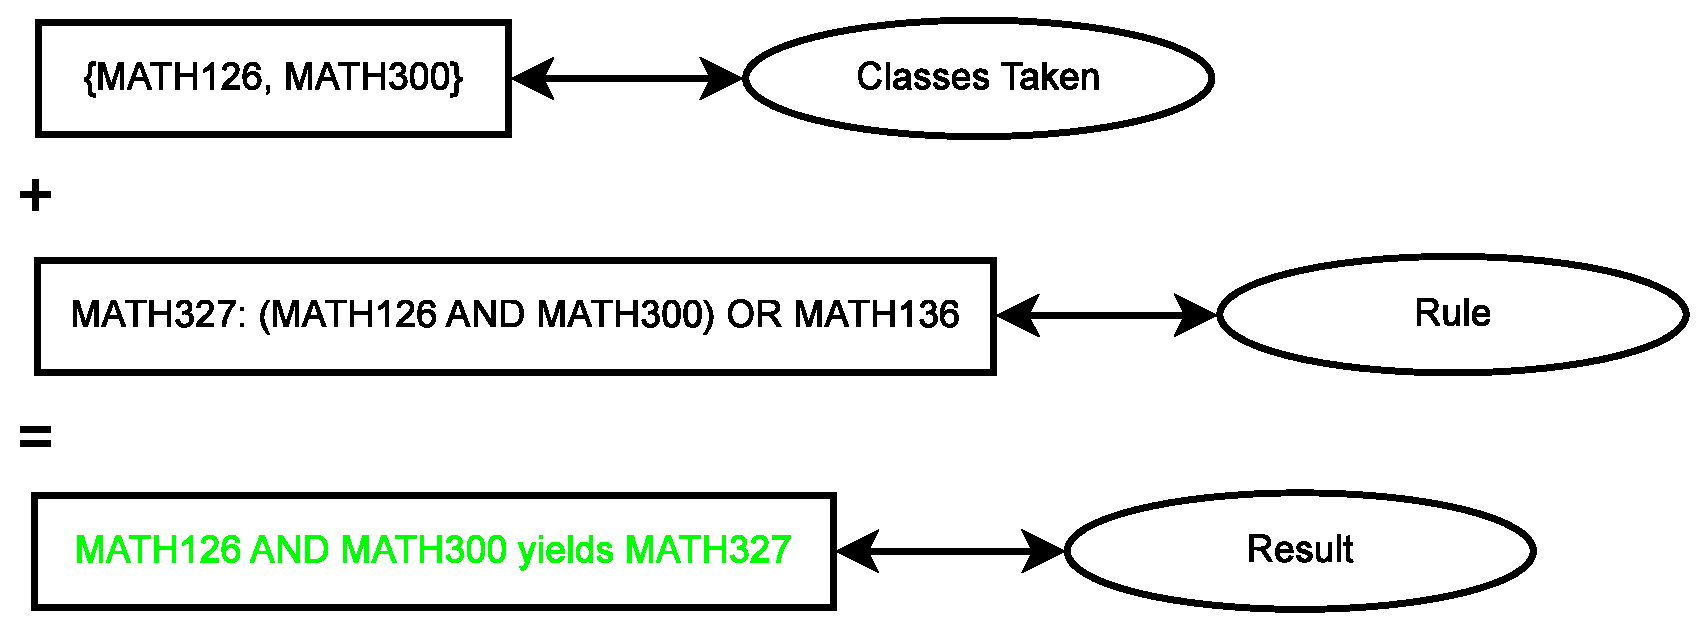
\includegraphics[scale=0.4]{prereq_logic_example} \end{center}
\caption{Evaluation of a rule} \label{logic_ex} \end{figure}

To represent alternative and multiple prerequisites we introduced a set of logic
rules for each course. The prerequisites for each course are expressed as
propositional logic statements stored in the set $R$. The literal propositions
in each rule are related to whether or not a student has taken a particular
course. For example, the rule associated with $MATH327$ in fig~\ref{logic_ex} is
$$ \text{{\it MATH327: (MATH126 AND MATH300) OR MATH136}}.$$

To determine if a given student is eligible to register for a course offering,
c we can evaluate the rule for c. Each literal proposition in the rule takes on
the value true if a student has already taken the course, and false if he or she
hasn't.  If the rule evaluates to true, then the student is eligible to take the
course; otherwise. For example, consider Figure~\ref{logic_ex}, here a student
has previously taken courses $MATH126$ and $MATH300$. Since $MATH126$ and
$MATH300$ have been taken, then those literals in the rule for $MATH327$
evaluate to true and therefore the entire rule is true.  Since the entire rule
is true, the student can take $MATH327$.

\subsection{Initial Model and Tractability} With a static schedule it would be
possible to plan an entire set of quarter by quarter schedules from start to
finish. Unfortunately we have neither the computational resources nor the luxury
of a static schedule. Some classes are offered every quarter others such as
senior electives are not. Furthermore for some classes it cannot be predicted
more than one quarter in advance when a senior elective will be offered. Even
given perfect information, where we know the possible class schedules for every
quarter we face another problem; finding the best possible schedule reduces to
enumerating possible class schedules for every quarter until the graduation
requirements are satisfied.  Given that we cannot predict in advance the
conflicts between classes, we cannot even determine the branching factor of the
enumeration tree nor its depth. Since we can only determine one quarter in
advance, this suggests approaching the problem by using heuristics to pick the
best possible classes each quarter.

Instead of trying to solve the complete problem we chose to use the "rolling
horizon approach" used by Xiangtong et al \cite{xiangton:informs} when
scheduling classes for airline pilots. Xiangtong et al. also could not develop
an optimal class schedule in one pass, instead they picked optimal classes based
using a heuristic over a well demarcated time period. Once they had a solution
to the smaller time period, they increase the size of the time period, or rolled
the horizon, and used the previously optimal solution to help determine
a solution to the new larger problem. The team's algorithm continued rolling the
time horizon on the problem until they had a solution to the entire problem.

\section{Picking Classes Per Quarter} Since determining an entire schedule at
once is intractable we adapted the rolling horizons approach which uses
a heuristic to pick the best possible schedule for a quarter. With a good
heuristic we will be able to choose classes that lead to a minimized graduation
time. Since we cannot analytically determine graduation time based on classes
chosen in a single quarter, our heuristic tries to give high value to classes
that would delay graduation is taken later rather than sooner. 

We break our algorithm down into two main phases: determining available course
offering and selecting specific course offerings.

\subsection{Determining Available Course Offerings} We need to select the
classes we can currently take and then build conflict graphs for classes based
on the times they are offered. The set $L_i$ is built in this part of the
algorithm.

\subsubsection{Procedure} We present the procedure for populating the set $L$ as
follows: \begin{enumerate} \item For each rule $r \in R$ we iterate over each
proposition $p$ in the rule. Recall that $p$ represents a course, for example
$MATH125$. We then check if $p \in T$.  If $p \in T$ then we say $p$ evaluates
to true; otherwise, $p$ evaluates to false.  Using rules of logic we evaluate
$r$, if $r$ true, then we add the course associated with it to $L$.  Once this
is complete, $L$ will consist of every course that could be taken based solely
on prerequisites that we have fulfilled.  \item We now prune $L$ by removing all
courses that are not offered in the current quarter. $L$ now only contain
classes that we can take given the current quarter and the classes we have
already taken.  \item We now construct a conflict graph, $G_{conflict}$, where
every course offering in $L$ is a node, and there is an edge between two nodes
$i$ and $j$ if and only if the time of course offering $i$ overlaps the time of
course offering $j$.  \end{enumerate}

\begin{figure} [ht]
    \begin{center}
        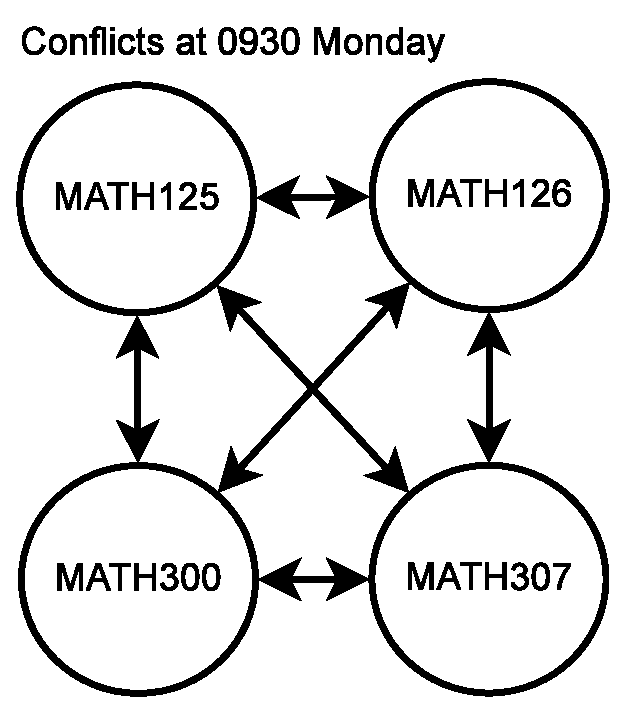
\includegraphics[scale=0.35]{conflict_graph_ex}
    \end{center}
    \caption{A Conflict Graph}
    \label{conflictg}
\end{figure}

\subsubsection{Analysis} The selection procedure involves a lot of set queries
and iteration, but in asymptotic running time the algorithm is relatively quick.
Let $n$ be the total number of classes ever available to take, or in other
words, $n = \|U\|$. In the worst case, $P$ has a complex rule for all $n$
courses, and checking each rule in $P$ is linear in the number of propositions.
However, we know {\it a priori} from analysis of our data set that the largest
rule has twelve propositions, so we can bound the rule check time by a constant,
$C$, and therefore step one can be done in $O(n)$ time.

Continuing to step two, the worst case is when $L$ = {all classes offered during
the quarter}.  Checking whether a course is offered in a given quarter can be
done in constant time, and we have $n$ courses to check, therefore step two can
also be done in $O(n)$ time.

Finally, the last step is once again bounded by a constant and $n$. Considering
courses between 8:30am and 7:30pm, we have nine fifty-minute time periods, and
five days of the week, and therefore we have 45 time slots to check in our
conflict graph, again yielding $O(n)$ runtime.

Since we are dealing with asymptotic running time we will drop the constant
terms and combining all results yields an overall runtime of $O(n)$.

\subsection{Selection of Quarterly Classes} To select classes we give each class
a value and weight. The primary problem is the the classes contained in $L$
almost certainly have time conflicts, likely between courses that need to be
taken. 

\subsubsection{Heuristic Value Function} In order to determine which classes
should be picked in a given schedule, we use a heuristic function which assigns
each class a value. The higher the value of this function for a class, the more
likely that class will be placed in the schedule.  Recalling that our goal is to
minimize the total number of quarters taken (and implicitly, maximize the total
number of courses taken per quarter).  Our heuristic function should give higher
value to class that maximize the number of classes taken this quarter and in
future quarters.  One component to the heuristic function then must be the
number of dependent courses a given course offering has. If a course satisfies
many prerequisites, then we know that there are many courses that we cannot
complete without it, so we want our heuristic function to favor it. 

Additionally, we know that not every course is offered every quarter. If
a course is not offered until the following year, we could potentially add an
entire year to the schedule. This is a situation we hope to avoid. Our heuristic
function must therefore consider how often and how far in the future a given
course is offered. For example, if we are deciding between two course offering
that are identical except one is offered once a year, and the other is offered
three times a year, we want to take the course only offered once a year, as we
won't have the opportunity to take it for another entire year.

\begin{figure} [ht]
    \begin{center}
        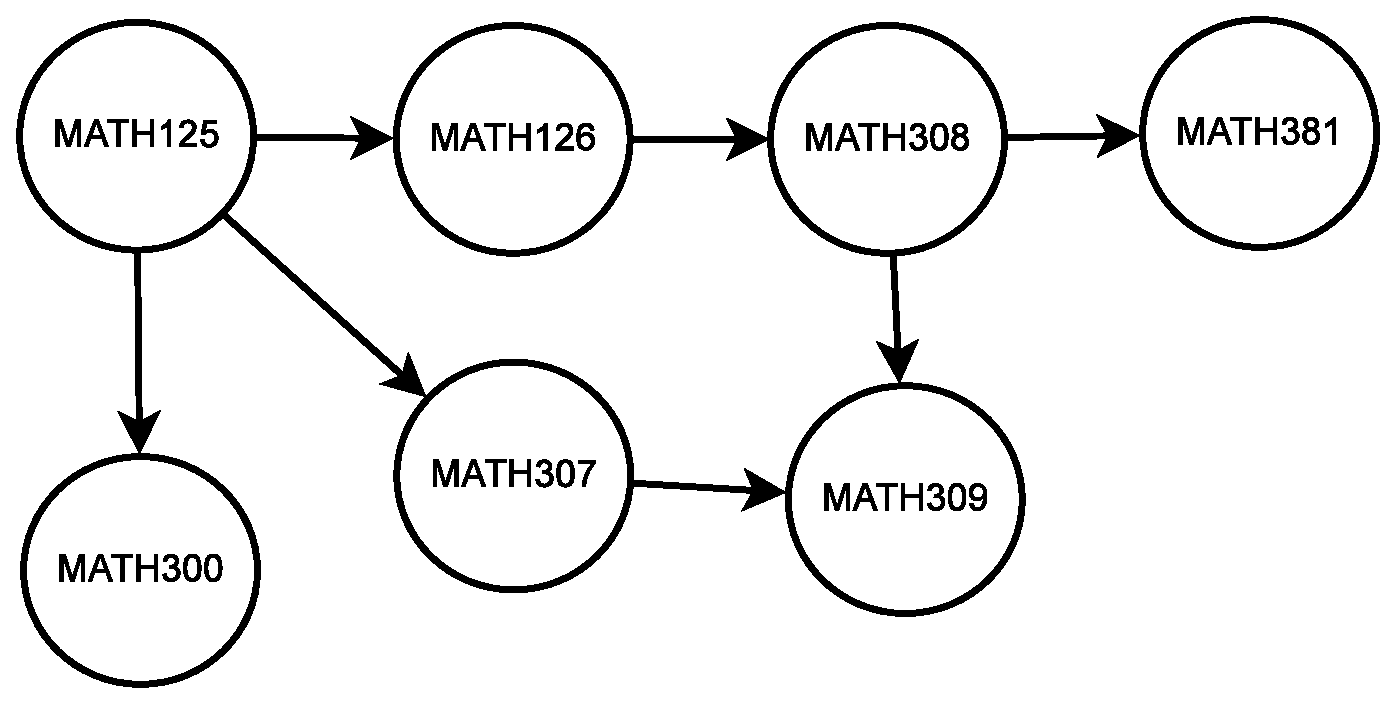
\includegraphics[scale=0.35]{more_prereq_tree}
    \end{center}
    \caption{A Prerequisite DAG}
    \label{prereq}
\end{figure}

We these considerations in mind, we begin to develop our heuristic function. In
order to define our heuristic function, we must first define some auxiliary
functions on course offering.  \begin{itemize} \item Let $TimeFromNow(c, q)$ be
difference in quarters between the current quarter, $q$, and the next quarter
a given course offering, $c$, is offered. As there are four quarters, the range
of this function is $\{0, 1, 2, 3\}$.  \item Let $Quarters(c)$ be the number of
quarters per year a given course, $c$, is offered. As there are four quarters,
the range of this function is $\{0, 1, 2, 3, 4\}$.  \item Let $Dependents(c)$ be
the number of course that either directly or indirectly require a given course,
$c$. In Figure~\ref{prereq}, $Dependents(MATH125)$ = 6 while
$Dependents(MATH307)$ = 1 \end{itemize}

With these functions defined, we can now define our heuristic function:

\begin{equation} 
    Value(c) = 1 + \alpha * Dependents(c) + \beta * TimeFromNow(c,q) 
    - \gamma * Quarters(c)
    \label{value_func}
\end{equation} 

Where $c$ is a given course offering, $q$ is the current quarter, and $\alpha$,
$\beta$, and $\gamma$ are real numbers, giving a weight to piece of the
heuristic. The scalars are determined experimentally.  

\subsubsection{Selection Procedure} At this point in the algorithm we know which
courses are available to a student and their relative values. We present two
ways of approaching quarterly class choice.  We will initially encode the class
selection as a binary integer programming problem in spirit of the methods
presented by Dinkel et al \cite{dinkel:scheduling}. and Pritsker et al
\cite{prisker:informs}. A second approach developed by Yamada et al
\cite{yamada:heuristic} and Pferschy et al \cite{pferschy:kcg} is presented for
dealing with very large class choices where binary LP would be difficult solve.

\subsubsection{Formulation as Binary Integer Program} We can now formulate
a binary linear programming problem. Before stating the linear
program, we must first define some variables used in it: 

\begin{itemize}
    \item $ X_i = \left\{ \begin{array}{lr} 1 \text{ if we take } X_i\\ 0 \text{ if
we don't take } X_i \end{array} \right. $ 
    \item For all $t \in O$, we let $t$ represent the conflict graph of classes
    at time period $t$.
    \item Let $m = \|L\|$.  
\end{itemize} 
We now state our problem as follows: 

Maximize: 
\begin{equation}
    \text{Value of Quarter} = \sum_{i=1}^m Value(c_i) * X_i
    \label{qtr_val}
\end{equation}
Subject To:
\begin{equation}
    \sum_{i=1}^m Weight(c_i) * X_i \leq l, 
    \label{weight_lim}
\end{equation}

\begin{equation}
    \forall t \in O,X_i+X_j \leq 1, \forall \text{ connected pairs } (X_i,X_j) \in t
    \label{time_con}
\end{equation}

\begin{equation}
   X_i + X_j \leq 1, \forall \text{ pairs } (X_i,X_j) \text{ where } X_i \text{and} X_j \text{ are offerings of
   the same course}
    \label{course_con}
\end{equation}

The linear program
can be interpreted as follows: \begin{itemize} \item The value of a quarter is
the total number of courses taken that quarter.  \item In each quarter, the
total number of credits cannot exceed the specified limit.  \item Only one
course can be taken in one particular time slot \item A course can only be taken
or not taken. In other words, decision variables are binary.  \item Each
non-zero decision variable in the optimal solution represents a class we will
take.  \end{itemize}

Each of the equations based on eqn.~\ref{time_con} ensure that we only take one class per 
time period per day. Also this linear program is ‘nice’ in that it always has 
feasible origin (don’t take any classes), and that the simplest formulation 
is already in standard form.

As noted in the reference literature this is actually a NP-hard
problem as described \cite{pferschy:kcg}. For versions of this problem in the
low hundreds of variables, however it is still possible to solve using modern LP
solving software \cite{yamada:heuristic}. In our case, just solving for the
optimal classes for a single major fits well into the scope of a few hundred (or
even just tens of) variables. For multiple majors or to consider class selection
for distribution and elective requirements, however the number of classes
balloons significantly and the KCG problem becomes much harder. For this version
of the problem we suggest the techniques used by Yamada et al
\cite{yamada:heuristic}, which we briefly outline below.

For the rest of this section we consider an alternative formulation of class
selection as a knapsack problem with conflict graphs and suggest the use
a technique developed by Yamada et. al.  \cite{yamada:heuristic}.

\subsubsection{Relaxation and Implicit Enumeration} \begin{enumerate} \item
Develop upper bound on value by solving a continuous version knapsack problem
generated by a Lagrangian relaxation of our problem. Let $X_i$ be a continuous
variable with $0 \leq X_i \leq 1$, and shift the time constraints into the
objective function by using a penalty of $\lambda$ when the constraint is
violated.  \item Use the upper bound developed above with the pruning rules
suggested by Yamada et al \cite{yamada:heuristic} to do implicit enumeration of
the possible choices.  \end{enumerate}

In Yamada et al’s \cite{yamada:heuristic} numerical runtime analysis they found
this algorithm ran very favorably against solving the same problem using popular
linear programming solvers. There is one problem that we should briefly address,
because the number of periods of available classes per week is relatively small
the conflict rate for a large number of class is relatively higher than Yamada
et al’s 2\% maximal conflict rate for their experiments. Our data has
a significant mitigating factor though, knapsack problems in general are
exponential in terms of the number of choices and the total weight capacity.
Realistically the total weight capacity is going to be 20 credits or less which
is between 1\% and 2\% of the figures used by Yamada \cite{yamada:heuristic} and
also our total number of choices is in many cases (particular just the classes
in a particular major) less than 200. Giving the size and type of data in our
set the higher conflict rate is less of a concern and Yamada et al’s algorithm
should still be efficient.

\section{Computational Results} In this section we will outline results obtained
by running computer simulations of schedule picking. We will computationally
examine what parameters in our heuristic function produce the most desirable
schedules.

\bibliography{paper_references}{} \bibliographystyle{plain} \end{document}
